\documentclass[12pt]{article}
\usepackage{amsmath, amssymb, amsthm, bm}
\usepackage{graphicx}
\usepackage{float}
\usepackage{geometry}
\usepackage{tikz}
\usetikzlibrary{arrows.meta, calc, positioning}
\usepackage{xcolor} 
\usepackage{enumitem}
\usepackage[skip=0.8em]{parskip}

\newtheorem{proposition}{Proposition}
\newtheorem{theorem}{Theorem}
\newtheorem{lemma}{Lemma}
\theoremstyle{definition}
    \newtheorem{definition}{Definition}[section]
    \newtheorem{condition}{Condition}
\theoremstyle{remark}
    \newtheorem{remark}{Remark}
\geometry{margin=1in}

\begin{document}


{\center{\LARGE On Admissibility of Tests for the iRelevant Paper}}\\
{June 25, 2026}

\section*{Basic Setup: Admissibility in the Normal Experiment}

Let $X \in \mathbf{R}^k$ denote a random vector distributed according to a multivariate normal distribution with mean $\mu$ and known, invertible covariance matrix $\Sigma$, that is,
\[
X \sim N(\mu, \Sigma), \quad \mu \in \Lambda := \mathbf{R}^k, \; \Sigma > 0~.
\]

We are interested in testing the composite null hypothesis
\begin{equation} \label{eq:null}
H_0 : \mu \in \Lambda_0 \quad \text{versus} \quad H_1 : \mu \in \Lambda_1 := \Lambda \setminus \Lambda_0~,
\end{equation}
where
\[
\Lambda_0 := \{ \mu \in \Lambda : \mu \le 0 \}, \qquad \Lambda_1 := \{ \mu \in \Lambda : \mu_j > 0 \text{ for some } j \}~.
\]

A test is a measurable function $\phi : \mathbf{R}^k \to [0,1]$, where $\phi(x)$ denotes the probability of rejecting $H_0$ given observation $x$.  The test $\phi$ satisfies the finite-sample size constraint
\begin{equation} \label{eq:size}
\sup_{\mu \in \Lambda_0} E_\mu[\phi(X)] \leq \alpha~,
\end{equation}
for some pre-specified level $\alpha \in (0,1)$.

Because the sample mean $\bar X$ is a sufficient statistic for $\mu$ when the data are i.i.d. normal, we may, without loss of generality, set $n=1$ and work directly with the single observation $X$.

It is well known that there is no uniformly most powerful (UMP) test for \eqref{eq:null}.  Instead, one can study admissibility of tests satisfying \eqref{eq:size}.  Following Romano and Shaikh (2015), a test $\phi$ satisfying \eqref{eq:size} is:
\begin{itemize}
    \item \emph{$\alpha$-admissible} if for any other test $\tilde \phi$ satisfying \eqref{eq:size},
    \[
    E_\mu[\tilde \phi] \ge E_\mu[\phi] \text{ for all } \mu \in \Lambda_1
    \quad \Rightarrow \quad
    E_\mu[\tilde \phi] = E_\mu[\phi] \text{ for all } \mu \in \Lambda_1~;
    \]
    \item \emph{$d$-admissible} if for any other test $\tilde \phi$ satisfying \eqref{eq:size},
    \[
    E_\mu[\tilde \phi] \ge E_\mu[\phi] \text{ for all } \mu \in \Lambda_1, \quad
    E_\mu[\tilde \phi] \le E_\mu[\phi] \text{ for all } \mu \in \Lambda_0
    \quad \Rightarrow \quad
    E_\mu[\tilde \phi] = E_\mu[\phi] \text{ for all } \mu \in \Lambda~.
    \]
\end{itemize}

Romano and Shaikh (2015) show that any test $\phi$ satisfying \eqref{eq:size} whose acceptance region is a closed, convex subset of $\mathbf{R}^k$ containing $\Lambda_0$ is $d$-admissible.  If, in addition, the supremum in \eqref{eq:size} is attained and the inequality holds with equality, then $\phi$ is also $\alpha$-admissible. However, there is no circulating paper so we cannot cite and so I decided to prove this result here as a preliminary result for the case that is relevant for our paper. 

\newpage 

\section*{The unrestricted case in the Normal location model}

\begin{theorem}[Closed convex acceptance regions imply admissibility]
    Let
    \[
    X\sim N(\mu,\Sigma)~,
    \]
    where $\Sigma$ is known and positive definite and $\mu\in\mathbf R^k$. Consider testing
    \[
    H_0:\mu\in\Lambda_0:=\{\mu:\mu\le 0\}
    \quad\text{versus}\quad
    H_1:\mu\in\Lambda_1:=\mathbf R^k\setminus\Lambda_0~,
    \]
    at level $\alpha \in (0,1)$.    Let $\phi_0$ be a nonrandomized test with acceptance region
    \[
    A_0:=\{x:\phi_0(x)=0\}~.
    \]
    Assume that $A_0$ is closed and convex and that $\phi_0$ has level $\alpha$; i.e, \eqref{eq:size} holds. Then 
    \begin{enumerate}
    \item $\phi_0$ is $d$-admissible for testing $H_0$ against $H_1$.
    \item If, in addition, there exists a finite point $\mu_0\in\Lambda_0$ such that
    \[
    E_{\mu_0}[\phi_0(X)]=\alpha~,
    \]
    then $\phi_0$ is $\alpha$-admissible.  
    \end{enumerate}
\end{theorem}
    
\begin{proof}
We use the following consequence of Theorem 6.7.1 and Corollary 6.7.1 of Lehmann and Romano.

\begin{proposition}[Lehmann--Romano]
Consider an exponential family with density
\[
p_\theta(t):=C(\theta)\exp\{\theta't\}
\]
with respect to a $\sigma$-finite measure $\nu$, with natural parameter space $\Omega$. Let $\Omega_H$ and $\Omega'$ be disjoint nonempty subsets of $\Omega$. Let $\phi_0$ be a nonrandomized test of $H:\theta\in\Omega_H$, based on $T$, with acceptance region $A_0\subseteq\mathbf R^s$. Suppose $A_0$ is closed and convex and that the following ray condition holds: whenever
\[
A_0\cap\{t:a't>c\}=\varnothing~,
\]
there exist $\theta^*\in\Omega$ and $\lambda_n\to\infty$ such that
\[
\theta^*+\lambda_n a\in\Omega'~.
\]
Then the test with acceptance region $A_0$ is $d$-admissible. If the test has size $\alpha$ and there exists a finite point $\theta_0\in\overline{\Omega_H}$ such that
\[
E_{\theta_0}[\phi_0(X)]=\alpha~,
\]
then the test is also $\alpha$-admissible. These admissibility conclusions allow randomized competing tests.
\end{proposition}

We now verify the assumptions of this result. Write the normal density in canonical exponential-family form. Let
\[
\theta :=\Sigma^{-1}\mu,
\qquad
\mu=\Sigma\theta~.
\]
With respect to the measure
\[
d\nu(x):=(2\pi)^{-k/2}|\Sigma|^{-1/2}
\exp\left\{-\frac12 x'\Sigma^{-1}x\right\}dx~,
\]
the density of $X\sim N(\Sigma\theta,\Sigma)$ is
\[
p_\theta(x):=\exp\left\{\theta'x-\frac12\theta'\Sigma\theta\right\}~.
\]
Thus $T(x):=x$, $\Omega:=\mathbf R^k$, and
\[
\Omega_H:=\{\theta:\Sigma\theta\le 0\},
\qquad
\Omega_K:=\{\theta:\Sigma\theta\not\le 0\}~.
\]
We apply the Lehmann--Romano result with $\Omega'=\Omega_K$.

It remains to verify the ray condition. Let $a\in\mathbf R^k$ and $c\in\mathbf R$ satisfy
\[
A_0\cap\{x:a'x>c\}=\varnothing~.
\]
If $a=0$, choose any $\theta^*\in\Omega_K$ and the condition is immediate.  Hence suppose $a\ne 0$. Equivalently, $A_0\subseteq\{x:a'x\le c\}$. We claim that
\[
\Sigma a\not\le 0~.
\]
Suppose instead that $\Sigma a\le 0$. For $\lambda>0$, define
\[
\theta_\lambda :=\lambda a,
\qquad
\mu_\lambda :=\Sigma\theta_\lambda=\lambda\Sigma a~.
\]
Then $\mu_\lambda\le 0$, so $\theta_\lambda\in\Omega_H$ for all $\lambda>0$. Under $P_{\theta_\lambda}$,
\[
a'X \stackrel{P_{\theta_\lambda}}{\sim} N\left(\lambda a'\Sigma a,\ a'\Sigma a\right)~.
\]
Since $\Sigma$ is positive definite and $a\ne 0$, $a'\Sigma a>0$. Hence
\[
P_{\theta_\lambda}(a'X>c)\to 1 \quad \text{as} \quad \lambda\to\infty~.
\]
Because $A_0\subseteq\{x:a'x\le c\}$, we have $\{x:a'x>c\}\subseteq A_0^c$. Since $\phi_0$ is nonrandomized,
\[
E_{\theta_\lambda}[\phi_0(X)] = P_{\theta_\lambda}(X\in A_0^c)
\ge P_{\theta_\lambda}(a'X>c)
\to 1 \quad \text{as} \quad \lambda\to\infty~.
\]
This contradicts the level condition because every $\theta_\lambda\in\Omega_H$ and $\alpha<1$. Therefore $\Sigma a\not\le 0$.

It follows that $\lambda\Sigma a = \Sigma(\lambda a)\not\le 0$ for every $\lambda>0$. Hence
\[
\lambda a\in\Omega_K
\qquad\text{for every }\lambda>0~.
\]
The ray condition holds with $\theta^*=0$ and any sequence $\lambda_n\to\infty$.

The Lehmann--Romano proposition therefore gives $d$-admissibility of $\phi_0$ against possibly randomized competitors.

Finally suppose there exists finite $\mu_0\in\Lambda_0$ such that $E_{\mu_0}[\phi_0(X)]=\alpha$. Let $\theta_0=\Sigma^{-1}\mu_0$. Then $\theta_0\in\Omega_H\subseteq\overline{\Omega_H}$ and
\[
E_{\theta_0}[\phi_0(X)]=\alpha~.
\]
The second part of the Lehmann--Romano corollary gives $\alpha$-admissibility, again against possibly randomized competitors.
\end{proof}

\begin{remark}
    Exact size is \emph{needed} for $\alpha$-admissibility. To see this, consider the zero test $\phi(x):=0$ with acceptance region $\mathbf R^k$, which is closed and convex, and it satisfies the size constraint for every $0<\alpha<1$. But it is not $\alpha$-admissible. The test
    \[
    \psi(x):=I\{x_1>\sqrt{\Sigma_{11}}\Phi^{-1}(1-\alpha)\}
    \]
    has level $\alpha$ for $H_0:\mu\le 0$ and has strictly positive power at alternatives with $\mu_1>0$, while the zero test has zero power everywhere.
\end{remark}


\section*{The restricted case: A simple race}
Before we study admissibility in the restricted parameter space case, we show that the short and long tests are mutually non-dominated on the restricted alternative $\Lambda_1$.

Let $X\sim N(\mu,I_2)$ with restricted parameter space
\[
\Lambda:=\{\mu:\mu_2\le\mu_1\},\qquad
\Lambda_0:=\{\mu\in\Lambda:\mu_1\le0\},\qquad
\Lambda_1:=\{\mu\in\Lambda:\mu_1>0\}~.
\]
Consider the two level-$\alpha$ tests
\[
\varphi_s(x):=I\{x_1>c_s\},\qquad
\varphi_\ell(x):=I\{\max(x_1,x_2)>c_\ell\}~,
\]
with
\[
c_s:=\Phi^{-1}(1-\alpha),\qquad
c_\ell:=\Phi^{-1}\!\big(\sqrt{1-\alpha}\big)~.
\]
Since $\sqrt{1-\alpha}>1-\alpha$ for $\alpha\in(0,1)$, we have $c_\ell>c_s$. Both tests are coordinatewise monotone, so their least favorable null point is $\mu=0$, where each has size exactly $\alpha$. Their power functions on $\Lambda_1$ are
\[
\beta_s(\mu):=\Phi(\mu_1-c_s),\qquad
\beta_\ell(\mu):=1-\Phi(c_\ell-\mu_1)\,\Phi(c_\ell-\mu_2)~.
\]
The short power depends on $\mu_1$ only; the long power is symmetric and coordinatewise increasing.

\begin{proposition}
For every $\alpha\in(0,1)$, neither $\varphi_s$ nor $\varphi_\ell$ dominates the other on $\Lambda_1$.
\end{proposition}

\begin{proof}
\emph{Short wins for $\mu_2\ll\mu_1$.} Fix $\mu_1>0$ and let $\mu_2\to-\infty$. Then $\Phi(c_\ell-\mu_2)\to1$, so
\[
\beta_\ell(\mu)\to 1-\Phi(c_\ell-\mu_1)=\Phi(\mu_1-c_\ell)~,
\]
and since $c_\ell>c_s$,
\[
\beta_s(\mu)-\beta_\ell(\mu)\ \longrightarrow\ \Phi(\mu_1-c_s)-\Phi(\mu_1-c_\ell)\ >\ 0~.
\]
Hence $\beta_s>\beta_\ell$ for $\mu_2$ sufficiently small.

\emph{Long wins near the diagonal.} On $\mu_1=\mu_2=t$,
\[
g(t):=\beta_\ell(t,t)-\beta_s(t,t)=\Phi(c_s-t)-\Phi(c_\ell-t)^2~,
\]
where $\Phi(c_s-t)=1-\beta_s$ and $\Phi(c_\ell-t)^2=1-\beta_\ell$ are the two tests' miss probabilities; thus $g(t)>0$ iff the long test misses less often. The two miss probabilities decay at different rates. By Mills' ratio, $\Phi(-z)\sim\phi(z)/z$ as $z\to\infty$, so
\[
\log\Phi(c_s-t)=-\tfrac12(t-c_s)^2+O(\log t),
\qquad
\log\Phi(c_\ell-t)^2=-(t-c_\ell)^2+O(\log t)~,
\]
the second rate being twice the first because the long test misses only when \emph{both} coordinates fall short. Subtracting,
\[
\log\frac{\Phi(c_\ell-t)^2}{\Phi(c_s-t)}
=-(t-c_\ell)^2+\tfrac12(t-c_s)^2+O(\log t)
=-\tfrac12 t^2+O(t)\ \longrightarrow\ -\infty~,
\]
so the ratio tends to $0$. Hence $\Phi(c_\ell-t)^2<\Phi(c_s-t)$, i.e.\ $\beta_\ell(t,t)>\beta_s(t,t)$, for all large $t$.
 
The two regions are nonempty for every $\alpha\in(0,1)$, which proves the claim.
\end{proof}

\begin{figure}[H]
\centering
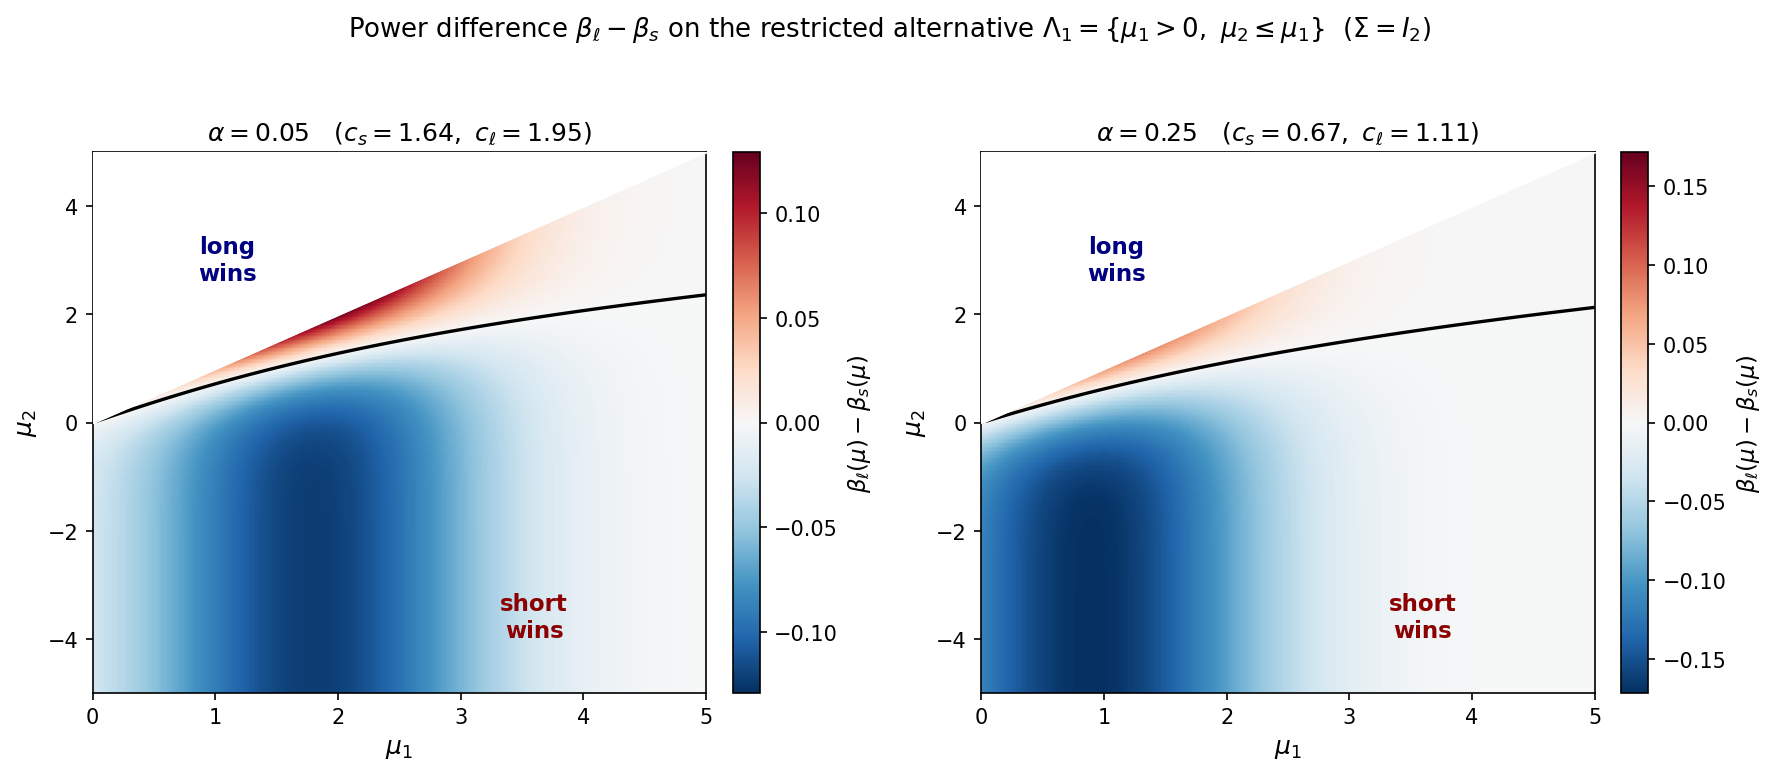
\includegraphics[width=\textwidth]{short_vs_long.png}
\caption{Power difference $\beta_\ell-\beta_s$ on $\Lambda_1=\{\mu_1>0,\ \mu_2\le\mu_1\}$ for $\alpha=0.05$ and $\alpha=0.25$. The black curve is the crossover $\beta_\ell=\beta_s$. The short test wins in the interior of the cone ($\mu_2$ well below $\mu_1$); the long test wins near the boundary $\mu_2\approx\mu_1$.}
\end{figure}


\section*{The Restricted case in the Normal location model}
The restricted problem is genuinely different. Restricting $\Lambda$ to $\mu_2\le \mu_1$ shrinks the alternative $\Lambda_1$, and that does two things at once: it breaks the LR ray condition (some support directions of a convex $A_0$ no longer reach the alternative), and, perhaps more consequentially, it creates new dominators, because a competitor now only has to win on the smaller $\Lambda_1$. This is illustrated in Federico's result and in a new result below. Relatedly, a previous counterexample I wrote shows that the test $\phi_{\delta}(x):=I\{x_2-x_1 > c\}$ is dominated and so it breaks the sufficiency of closed and convex acceptance regions: the acceptance region of this test is closed, convex, level $\alpha$, but it aims rejection mass at $\mu_2-\mu_1 > 0$, a region the restriction deleted, so the short test dominates it. Convexity alone is therefore genuinely insufficient.

\noindent
\boxed{%
\begin{minipage}{0.95\textwidth}
{\bf Executive summary.} We can summarize our results as follows:
\begin{enumerate}
\item The short test is globally {\bf admissible}.
\item The long test is globally {\bf inadmissible}.
\item Both are {\bf admissible} within the class of rectangular tests.
\item Rectangular tests are {\bf inadmissible} within the class $\mathcal C$ of tests that satisfy two monotonicities. Importantly, they are dominated by what we call the {\bf gated test}.
\item The gated test uses information from $X_1$ {\bf and} $X_2$ and is {\bf globally admissible}.
\item The gated test satisfies all of the assumptions in Andrews and Soares, except for Assumption 3: $S(m,\Omega)>0 \iff m_j<0\text{ for some inequality }j$.
\end{enumerate}
\end{minipage}%
}
\subsection*{The short test is globally admissible}
The previous section shows that the short and long tests are mutually non-dominated on the restricted alternative $\Lambda_1$. This result, however, does not directly speak to the question of admissibility of these test. Indeed, we will show that the short test is admissible without any class restrictions.

For simplicity consider the case $\Sigma=I_2$ and let $X\sim N(\mu,I_2)$ with restricted parameter space
\[
\Lambda:=\{\mu:\mu_2\le\mu_1\},\qquad
\Lambda_0:=\{\mu\in\Lambda:\mu_1\le0\},\qquad
\Lambda_1:=\{\mu\in\Lambda:\mu_1>0\}~.
\]
 
We invoke the Lehmann--Romano proposition previously stated (based on Theorem 6.7.1 / Corollary 6.7.1).
 
\begin{lemma}
For every $\alpha\in(0,1)$, the short test $\varphi_s$ is $\alpha$-admissible for testing $H_0$ against $H_1$ among all level-$\alpha$ tests, including randomized competitors. No restriction on the competing class is required.
\end{lemma}
 
\begin{proof}
Since $\Sigma=I_2$, $\theta=\mu$ and the model is the canonical exponential family $p_\theta(x)=\exp\{\theta'x-\tfrac12\|\theta\|^2\}$ relative to $N(0,I_2)$, with $T(x)=x$ and $\Omega=\mathbf R^2$; hence $\Omega'=\Lambda_1$.
 
\emph{Closed convex, exact size.} $A_s=\{x_1\le c_s\}$ is closed and convex. Since $E_\mu[\varphi_s]=\Phi(\mu_1-c_s)$ depends only on $\mu_1$ and is nondecreasing in it, and every $\mu\in\Lambda_0$ has $\mu_1\le0$,
\[
\sup_{\mu\in\Lambda_0}E_\mu[\varphi_s]=\Phi(-c_s)=\alpha~,
\]
attained at the finite null point $\mu_0=0\in\Lambda_0$.
 
\emph{Ray condition.} Suppose $a\ne0$ and $A_s\subseteq\{x:a'x\le c\}$, i.e.\ $\sup_{x\in A_s}a'x<\infty$. The set $A_s$ contains $(c_s,x_2)$ for every $x_2\in\mathbf R$ and $(x_1,0)$ for every $x_1\le c_s$; finiteness of the supremum therefore forces $a_2=0$ and $a_1\ge0$, and with $a\ne0$ this gives $a=a_1(1,0)$, $a_1>0$. Take $\theta^*=0$ and any $\lambda_n\to\infty$. Then
\[
\theta^*+\lambda_n a=(\lambda_n a_1,\,0)~,
\]
whose first coordinate $\lambda_n a_1>0$ satisfies $0\le\lambda_n a_1$, so the point lies in $\Lambda_1=\Omega'$. The ray condition holds.
 
By the Lehmann--Romano proposition, $\varphi_s$ is $d$-admissible against randomized competitors; since its size $\alpha$ is attained at $\mu_0=0$, it is $\alpha$-admissible. 
\end{proof}

\subsection*{The long test is globally inadmissible}

For $\varphi_\ell(x)= I\{\max(x_1,x_2)>c_\ell\}$ with $A_\ell=\{x_1\le c_\ell,\,x_2\le c_\ell\}$, the face $x_2=c_\ell$ yields the support direction $a=(0,1)$ with $A_\ell\subseteq\{x_2\le c_\ell\}$. For this $a$ no anchor $\theta^*$ admits a sequence $\lambda_n\to\infty$ with $\theta^*+\lambda_n(0,1)\in\Lambda_1$: the second coordinate $\theta^*_2+\lambda_n\to\infty$ while the first stays fixed, so $\mu_2\le\mu_1$ eventually fails. The ray condition is violated and the proposition is silent --- consistent with the fact (shown by counterexample) that $\varphi_\ell$ is not admissible without a class restriction. Equivalently, under $\Sigma=I_2$ a support direction $a$ is reachable in $\Lambda_1$ iff $a_2\le a_1$; the short test's only support direction $(1,0)$ satisfies this, the long test's direction $(0,1)$ does not.

I have a proof of this result and Federico also has a dominating test. May include later, but the result is that the long test is globally inadmissible.  


\section*{The Class of Rectangular Tests}
 
For cutoffs $c=(c_1,c_2)\in \overline{\mathbf R}^2$, define the rectangular acceptance region
\[
A_c:=\{x\in\mathbf R^2:x_1\le c_1,\ x_2\le c_2\}~,
\]
and the associated nonrandomized test
\[
\phi_c(x):= I \{x\notin A_c\}
=I \{x_1>c_1\text{ or }x_2>c_2\}~.
\]
The case $(c_1,c_2)=(c_s,\infty)$ is allowed; it gives the short test based only on $X_1$.  The case $c_1=c_2=\infty$ is the zero test, and the case  $(c_1,c_2)=(c_{\ell},c_{\ell})$ is the long test.
 
The ordered rectangular class is the class of such tests satisfying
\[
c_1\le c_2~.
\]
This is exactly the rectangle version of the order-respecting priority condition: coordinate 1 receives a weakly lower rejection cutoff than coordinate 2.
 
\subsection*{Admissibility of ordered rectangles within the class}
For $\mu\in\Lambda$, the acceptance probability is
\begin{equation}\label{eq:miss-probability}
    M_c(\mu):=
    P_\mu(X\in A_c)
    =
    \Phi(c_1-\mu_1)\Phi(c_2-\mu_2)~,
\end{equation}
and the power is
\[
\beta_c(\mu) := E_\mu[\phi_c(X)] = 1-M_c(\mu)~.
\]
For every $\mu\in\Lambda_0$, we have $\mu_1\le0$ and $\mu_2\le0$, hence
\[
M_c(\mu) = \Phi(c_1-\mu_1)\Phi(c_2-\mu_2) \ge \Phi(c_1)\Phi(c_2)~.
\]
Therefore
\[
\sup_{\mu\in\Lambda_0}E_\mu[\phi_c(X)] = 1 - \Phi(c_1)\Phi(c_2)~,
\]
with the supremum attained at the least favorable null point $\mu=0$. Consequently, $\phi_c$ has level at most $\alpha$ if and only if 
\begin{equation}\label{eq:level-constraint}
\Phi(c_1)\Phi(c_2)\ge \gamma := 1-\alpha~,
\end{equation}
and has exact size $\alpha$ if and only if equality holds.
 
Define the class of all rectangular level-$\alpha$ tests by
\[
\mathcal R_{\le\alpha}
:=
\{\phi_c:\Phi(c_1)\Phi(c_2)\ge \gamma\}~,
\]
the subclass of all level-$\alpha$ ordered rectangles by
\[
\mathcal R^{\mathrm{ord}}_{\le\alpha}
:=
\{\phi_c:c_1\le c_2,\ \Phi(c_1)\Phi(c_2)\ge \gamma\}~,
\]
and the subclass of all exact-size level-$\alpha$ ordered rectangles by
\[
\mathcal R^{\mathrm{ord}}_{\alpha}
:=
\{\phi_c:c_1\le c_2,\ \Phi(c_1)\Phi(c_2)= \gamma\}~.
\]
Admissibility below is relative to the class
$\mathcal R_{\le\alpha}$ of all rectangular level-$\alpha$ tests.
Specifically, an exact-size ordered rectangle
$\phi_c\in\mathcal R^{\mathrm{ord}}_{\alpha}$ is admissible relative to
$\mathcal R_{\le\alpha}$ if there is no
$\phi_d\in\mathcal R_{\le\alpha}$ such that
\[
\beta_d(\mu)\ge \beta_c(\mu)
\qquad\text{for every }\mu\in\Lambda_1~,
\]
with strict inequality for at least one $\mu\in\Lambda_1$.
Thus, the maintained test is required to be ordered, but the competing
rectangle is not. This is $\alpha$-admissibility relative to the rectangular class
$\mathcal R_{\le\alpha}$, rather than $\alpha$-admissibility among all
level-$\alpha$ tests.
 
\begin{theorem}[Exact-size ordered rectangles are admissible among all rectangles]\label{thm:ordered-rectangle-admissibility}
    Let $X\sim N_2(\mu,I_2)$ with
    \[
    \Lambda=\{\mu:\mu_2\le\mu_1\},
    \qquad
    \Lambda_1=\{\mu\in\Lambda:\mu_1>0\}.
    \]
    Fix $\alpha\in(0,1)$ and let $\phi_c\in\mathcal R^{\mathrm{ord}}_{\alpha}$, so
    \[
    c_1\le c_2,
    \qquad
    \Phi(c_1)\Phi(c_2)=1-\alpha.
    \]
    Then $\phi_c$ is admissible relative to $\mathcal R_{\le\alpha}$: if $\phi_d\in\mathcal R_{\le\alpha}$ satisfies
    \[
    E_\mu[\phi_d(X)]\ge E_\mu[\phi_c(X)]
    \qquad\text{for every }\mu\in\Lambda_1,
    \]
    then $\phi_d=\phi_c$ up to $P_\mu$-null sets for every $\mu$.
\end{theorem}
 
\begin{proof}
Let $\phi_d\in\mathcal R_{\le\alpha}$ dominate $\phi_c$ on $\Lambda_1$, with cutoffs $d=(d_1,d_2)$. The level characterization \eqref{eq:level-constraint} makes no use of ordering, so
\begin{equation}\label{eq:d-level}
\Phi(d_1)\Phi(d_2)\ge\gamma,
\end{equation}
and we do \emph{not} assume $d_1\le d_2$. By \eqref{eq:miss-probability}, domination $E_\mu[\phi_d]\ge E_\mu[\phi_c]$ on $\Lambda_1$ is equivalent to a weakly smaller miss probability:
\begin{equation}\label{eq:miss-domination}
M_d(\mu)=\Phi(d_1-\mu_1)\Phi(d_2-\mu_2)\ \le\ \Phi(c_1-\mu_1)\Phi(c_2-\mu_2)=M_c(\mu)
\qquad\text{for every }\mu\in\Lambda_1.
\end{equation}
We show $d=c$.
 
\emph{Step 1: exact size.}
If $\Phi(d_1)\Phi(d_2)>\gamma$, then
\[
M_d(0,0)=\Phi(d_1)\Phi(d_2)>\gamma=\Phi(c_1)\Phi(c_2)=M_c(0,0),
\]
so by continuity $M_d(t,t)>M_c(t,t)$ for all small $t>0$, with $(t,t)\in\Lambda_1$, contradicting \eqref{eq:miss-domination}. Hence $\phi_d$ has exact size,
\begin{equation}\label{eq:d-exact}
\Phi(d_1)\Phi(d_2)=\gamma.
\end{equation}
 
\emph{Step 2: the first cutoff satisfies $d_1\le c_1$.}
Fix $s>0$ and set $\mu=(s,r)$ with $r\le s$. Letting $r\to-\infty$ in \eqref{eq:miss-domination}, with $\Phi(d_2-r)\to1$ and $\Phi(c_2-r)\to1$, gives $\Phi(d_1-s)\le\Phi(c_1-s)$ for every $s>0$. Since $\Phi$ is strictly increasing,
\begin{equation}\label{eq:first-cutoff-order}
d_1\le c_1.
\end{equation}
This is the key use of the restricted alternative: sending the lower-priority mean $\mu_2$ to $-\infty$ exposes the first-coordinate cutoff.
 
\emph{Step 3: a strict drop is impossible, so $d_1=c_1$.}
Suppose, toward a contradiction, that $d_1<c_1$. If $c_2=\infty$, then $\Phi(c_2)=1$ and exact size \eqref{eq:d-exact} would force $\Phi(d_2)=\gamma/\Phi(d_1)>\gamma/\Phi(c_1)=1$, which is impossible; hence $c_2<\infty$. The same computation gives
\[
\Phi(d_2)=\frac{\gamma}{\Phi(d_1)}>\frac{\gamma}{\Phi(c_1)}=\Phi(c_2),
\qquad\text{so}\qquad d_2>c_2.
\]
In particular $d_1<c_1\le c_2<d_2$, so the competitor is itself ordered and the arc below stays in $\{x\le y\}$.
We record a monotonicity of the cutoff sum along the size curve $\Phi(x)\Phi(y)=\gamma$. Write $H:=\phi/\Phi$ for the reverse hazard rate; since $\Phi$ is log-concave, $H=(\log\Phi)'$ is strictly decreasing. The equation $\Phi(x)\Phi(y)=\gamma$ defines $y$ implicitly as a function of $x$. Differentiating both sides in $x$, with $y=y(x)$ and $\Phi'=\phi$, the chain rule gives
\[
\phi(x)\Phi(y)+\Phi(x)\,\phi(y)\,y'(x)=0~.
\]
Solving for $y'(x)$ and dividing numerator and denominator by $\Phi(x)\Phi(y)$ to expose $H=\phi/\Phi$,
\[
y'(x)=-\frac{\phi(x)\Phi(y)}{\Phi(x)\phi(y)}
=-\frac{\phi(x)/\Phi(x)}{\phi(y)/\Phi(y)}
=-\frac{H(x)}{H(y)}~.
\]
Adding the $1$ from differentiating $x$,
\[
\frac{d}{dx}\bigl(x+y\bigr)=1+y'(x)=1-\frac{H(x)}{H(y)}=\frac{H(y)-H(x)}{H(y)}~.
\]
Since $H(y)>0$, the sign of this derivative is the sign of $H(y)-H(x)$.
On this arc $x\le y$, so $H(x)\ge H(y)$ and the derivative is $\le0$, strictly negative once $x<y$. Hence lowering the first cutoff strictly raises the sum:
\begin{equation}\label{eq:cutoff-sum}
d_1+d_2>c_1+c_2.
\end{equation}
Now compare on the diagonal $\mu=(t,t)\in\Lambda_1$. By Mills' ratio, $\log\Phi(a-t)=-\tfrac12(t-a)^2-\log(t-a)+O(1)$ as $t\to\infty$; the constant and logarithmic terms cancel across the four factors, leaving
\[
\log\frac{M_d(t,t)}{M_c(t,t)}
=\sum_{j=1,2}\bigl[\log\Phi(d_j-t)-\log\Phi(c_j-t)\bigr]
=\bigl[(d_1+d_2)-(c_1+c_2)\bigr]\,t+O(1).
\]
By \eqref{eq:cutoff-sum} the leading coefficient is positive, so the ratio tends to $+\infty$; in particular $M_d(t,t)>M_c(t,t)$ for all large $t$, contradicting \eqref{eq:miss-domination}. (If $d_2=\infty$ the contradiction is immediate, since $M_d(t,t)/M_c(t,t)=\Phi(d_1-t)/[\Phi(c_1-t)\Phi(c_2-t)]\to\infty$ because $\Phi(c_2-t)\to0$.) Therefore $d_1=c_1$.
\end{proof}
 
\begin{remark}
The competitor $\phi_d$ is never assumed ordered: the priority condition $c_1\le c_2$ restricts only the maintained test, and domination supplies the rest. A strictly unordered rectangle cannot dominate at all---if $d_2<d_1$, then Step~2 gives $d_2<d_1\le c_1\le c_2$, so $\Phi(d_1)\Phi(d_2)<\Phi(c_1)\Phi(c_2)=\gamma$ violates the level constraint---while any competitor with $d_1<c_1$ is pushed by exact size into the ordered region $d_1<c_1\le c_2<d_2$, exactly where Step~3 operates. The same two limits also show that any two distinct exact-size ordered rectangles are mutually non-dominating: relabelling so that $d_1<c_1$, the competitor wins in the interior of the cone (Step~2) and loses on the far diagonal (Step~3).
\end{remark}

\[
\boxed{
\phi_c\text{ is admissible among all level-}\alpha\text{ rectangles}
\iff
\Phi(c_1)\Phi(c_2)=1-\alpha
\ \text{and}\
c_1\le c_2~.
}
\]

\subsection*{Inadmissibility of ordered rectangles within a restricted class}

A test $\phi=I\{x\notin A\}$ belongs to class $\mathcal C$ if its acceptance region satisfies:
\begin{itemize}[leftmargin=2.2em]
\item[\textbf{(M1)}] \emph{Coordinatewise monotonicity}: $A$ is a lower set, i.e.\ $x\le y$ and $y\in A$ imply $x\in A$. Equivalently $\phi$ is nondecreasing in each coordinate.
\item[\textbf{(M2)}] \emph{Order-respecting priority of coordinate $1$}: if $x_1\ge x_2$ and $x\in A$, then $ x_{\sigma}\in A$ (a permutation of the coordinates). Equivalently $\phi(x_1,x_2)\ge\phi(x_2,x_1)$ whenever $x_1\ge x_2$.
\end{itemize}
We write $\mathcal C_{\le\alpha}$ for the members of level $\le\alpha$, and $\mathcal C_{\alpha}$ for those of exact size $\alpha$. The ordered rectangles are exactly the rectangular members of $\mathcal C$.

It turns out that every exact-size ordered rectangle with a finite second cutoff is strictly dominated on
\[
\Lambda_1=\{\mu:\mu_1>0,\ \mu_2\le\mu_1\}
\]
by another exact-size test whose acceptance region is closed, convex, coordinatewise lower, and order-respecting.  The long test is therefore inadmissible relative to the proposed class.

The dominator has acceptance region
\[
    A_{c,b}:=\{x_1\le c,\ x_1+x_2\le b\},
\]
It keeps the coordinate-$1$ cutoff but replaces the low-priority coordinate cutoff $x_2\le c_2$ by a feasible aggregate cutoff $x_1+x_2\le b$. This test treats $X_1$ as the high-priority coordinate and $X_2$ as the low-priority coordinate. We call this test the ``gate the $X_2$ rejection by the value of $X_1$'' test; or ``gated'' test for short. 

To understand how to find the unique $b$ for a given $c$, consider the following. For a fixed first-coordinate gate \(c\), there is a unique finite \(b=b(c)\)
satisfying exact size iff
\[
\Phi(c)>\gamma,
\qquad\text{i.e.}\qquad
c>c_s:=\Phi^{-1}(\gamma).
\]
At the endpoint \(c=c_s\), the exact-size solution is \(b=\infty\), which gives
the short test. Thus the exact-size gated family can be indexed by
\[
c\in[c_s,\infty],
\qquad
b=b(c),
\]
with
\[
b(c_s)=\infty,
\qquad
\lim_{c\to\infty} b(c)=\sqrt 2\,\Phi^{-1}(\gamma)=\sqrt 2\,c_s .
\]
Moreover, \(b(c)\) is strictly decreasing in \(c\): relaxing the gate \(x_1\le c\)
requires tightening the diagonal cutoff \(x_1+x_2\le b\).

Equivalently, for a fixed diagonal cutoff \(b\), there is a unique finite
\(c=c(b)\) satisfying exact size iff
\[
P_0(X_1+X_2\le b)>\gamma,
\qquad\text{i.e.}\qquad
b>\sqrt 2\,c_s .
\]
At the endpoint \(b=\sqrt 2\,c_s\), the solution is \(c=\infty\), which gives
the pure diagonal-sum test \(I\{X_1+X_2>\sqrt 2\,c_s\}\).

 

%  - - - - - - - - - - - - - -- 
    \begin{thebibliography}{9}

\bibitem{LehmannRomano2005}
Lehmann, E. L. and Romano, J. P. (2005).
\textit{Testing Statistical Hypotheses}.
Third edition. Springer.

\end{thebibliography}

\end{document}
